\section{Modification of Valiant's algorithm}

In this section we describe the modification of Valiant's algorithm, which has a number of advantages, such as possibility to broke it down into several subtasks that can be processed independently. Also this version can be simply applied to the string-matching problem, which often arises in text editing, DNA and RNA sequence analysis.

\subsection{New approach}

The main change of this modification is the possibility to divide the parsing table into layers of disjoint submatrices of the same size. The division we have made from the reorganization of the matrix multiplication order is presented in \textbf{Figure 2}.  The layers are computed successively from the bottom up.

\begin{figure}[h]
\includegraphics[width=250pt]{layers2.eps}
\centering
\caption{Matrix partition on V-shaped layers.} \label{fig1}
\end{figure}

Let us consider the pseudo-code of the modification, which is written in \textbf{Algorithm 2}. The procedure $main()$ computes the lowest layer $(T_{l, l+1})$, and then divide the table into layers, described earlier, and computes them through the \textit{completeVLayer()} call. Thus, $main()$ computes all elements of parsing table $T$ correctly.

For the sake of brevity, we introduce \textit{left(m), right(m), top(m), bottom(m), rightgrounded(m)} and \textit{leftgrounded(m)} functions which returns the nessesary submatrix for matrix $m = (l, m, l', m')$ according to \textbf{Figure 1}.

Denote some subsidiary functions for matrix layer $M$:
 \begin{itemize}
  \item $bottomsublayer(M) = \{bottom(m) | m \in M \}$,
  \item \textit{lrsublayer(M)}$ = \{\textit{left(m)} | m \in M \} \cup \{\textit{right(m)} | m \in M \}$,
  \item $topsublayer(M) = \{top(m) | m \in M \}$.
\end{itemize}

The procedure \textit{completeVLayer(M)} takes an array of disjoint submatrices $M$.
For each $m = (l, m, l', m') \in M$ this procedure computes \textit{left(m), right(m), top(m)}.
The procedure assumes that the elements of $bottom(m)$ and all $T_{i, j} \forall l \leq i < j < m,  l' \leq i < j < m'$ are already constructed.
Also it is assumed that the current value of  $P[i, j] =  \{ (B, C) |\exists (m \le k < l'): a_{i + 1} \dots a_{k} \in L(B), a_{k + 1} \dots a_{j} \in L(C)\} \forall l \leq i < m,  l' \leq j < m'$.

The procedure \textit{completeLayer(M)} also takes an array of disjoint submatrices $M$, but unlike the previous one, it computes $T_{i, j} \forall (i, j) \in m$.
This procedure, just as in the previous case, assumes that  $T_{i, j} \forall l \leq i < j < m,  l' \leq i < j < m'$ are already constructed and the current value of  $P[i, j] =  \{ (B, C) |\exists (m \le k < l'): a_{i + 1} \dots a_{k} \in L(B), a_{k + 1} \dots a_{j} \in L(C)\}$ $\forall l \leq i < m,  l' \leq j < m'$.

% Algorithm2
\begin{algorithm}[t]
\SetAlgoNoLine
\KwIn{Grammar $G = (\Sigma, N, R, S), w = a_{1} \dots a_{n}, n \geq 1, a_{i} \in \Sigma$, where  n + 1 --- power of two}
\underline{main()}{:}{

 \For {$l \in \{1, \ldots, n \}$}{$T_{l, l + 1} = \{A | A \rightarrow a_{l + 1} \in R\}$}
 \For{$1 \le i < k $}{
 layer = $\textit{constructLayer(i)}$\;
 \textit{completeVLayer(layer)}
 }
 \BlankLine
 }

\underline{constructLayer(i)}{:}{
 \BlankLine
 $\{B | \exists k \geq 0 : B = (k*2^i, (k+1)*2^i, (k + 1)*2^i, (k+2)*2^i) \}$
 \BlankLine
    }
\underline{completeLayer(M)}{:}{
\BlankLine
\If {$\forall (l, m, l', m') \in M \quad (m - l = 1)$}{\For{$ (l, m, l', m') \in M$}{$T_{l, l'} = f(P_{l, l'})$\;}}
\Else{
\textit{completeLayer(bottomsublayer(M))}\;
\textit{completeVLayer(M)}
}
\BlankLine
}

\underline{comleteVLayer(M)}{:}{
 \BlankLine
 multiplicationTask1 = $\{left(subm), leftgrounded(subm), bottom(subm) | subm \in M \} \cup \linebreak  \{right(subm), bottom(subm), rightgrounded(subm) | subm \in M\}$\;
 \BlankLine
 multiplicationTask2 = $\{top(subm), leftgrounded(subm), right(subm) | subm \in M\}$\;
 \BlankLine
 multiplicationTask3 = $\{top(subm), left(subm), rightgrounded |subm \in M\}$\;
 \BlankLine
 \textit{performMultiplications(multiplicationTask1)}\;
 \textit{completeLayer(lrsublayer(M))}\;
 \textit{performMultiplications(multiplicationTask2)}\;
 \textit{performMultiplications(multiplicationTask3)}\;
 \textit{completeLayer(topsublayer(M))}

 }

\caption{Parsing by matrix multiplication: Modified Version}
\end{algorithm}

\textbf{Algorithm 3} describes how the procedure \textit{performMultiplication(task)}, where \textit{task} is an array of a triple of submatrices, works. It is worth mentioning that, as distinct from the original algorithm, $|tasks| \ge 1$ and all these multiplications can be computed independently.


 % Algorithm3
\begin{algorithm}[h]
\SetAlgoNoLine
\underline{performMultiplication(task)}{:}{\\
\For{$ (m, m1, m2) \in M$}{$P_{m} = P_{m} \cup (T_{m1} \times T_{m2})$\;}
}
\caption{}
\end{algorithm}

\subsection{Proof of correctness}

We provide the proof of correctness and time complexity for the proposed modification in this section.

\begin{theorem}
Let $M$ be a submatrix array. Assume that $T[i, j] =  \{ A |  a_{i + 1} \dots a_{j} \in L(A)\}$ $\forall l \leq i < j < m,  l' \leq i < j < m'$ and $P[i, j] =  \{ (B, C) |\exists (m \le k < l'): a_{i + 1} \dots a_{k} \in L(B), a_{k + 1} \dots a_{j} \in L(C)\}$ $\forall l \leq i < m,  l' \leq j < m'$ $\forall (l, m, l', m') \in M$.

Then the procedure \textit{completeLayer(M)}, returns correctly computed sets of $T[i, j]$ $\forall l \leq i \le m,  l' \leq j \le m'$ $\forall (l, m, l', m') \in M$.
\end{theorem}
%
% the environments 'definition', 'lemma', 'proposition', 'corollary',
% 'remark', and 'example' are defined in the LLNCS documentclass as well.
%
\begin{proof}
Induction on $\textit{m - l}$. (Hereinafter denoting $(l, m, l', m')$ as a typical example of array $M$, and all the computations are implemented for all submatrices in $M$).

The base case: $m - l = 1$. There is only one element to compute, and $P[l, l'] =  \{ (B, C) |  a_{l + 1} \dots a_{l'} \in L(B)L(C)\}$. Further, algorithm computes $f(P[l, l'])$ = \linebreak $\{ A |  a_{l + 1} \dots a_{l'} \in L(A)\}$, so $T[l, l']$ computed correctly.

For the induction step, assume that (l1, m1, l2, m2) is correctly computed for $m2 - l2 = m1 - l1 > m - l$.

Let us consider complete \textit{completeLayer(M)}, where $m - l > 1$.

Firstly, consider $\textit{completeLayer(bottom} = \{(\frac{l+m}{2}, m, l', \frac{l'+m'}{2})\})$, as theorem conditions are fulfilled, then this call returns correct sets $T[i, j]$ $\forall (i, j) \in bottom$ (hereinafter is means $\forall (i, j) \in m, \forall m \in \textit{bottom} $). All submatrices with size $ m1 - l1 > m - l $, all previous layers and also \textit{bottom(M)} are correct, so,  \textit{completeVLayer(M)} can be called, and \textit{multiplicationByTask(task1)} adds to each
$ P[i, j] \forall (i, j) \in left = \{(\frac{l+m}{2}, m, l', \frac{l'+m'}{2}))\} $
all pairs
$ \{(B, C) |\exists (\frac{l+m}{2} \le k < l'): a_{i + 1} \dots a_{k} \in L(B), a_{k + 1} \dots a_{j} \in L(C)\} $
 and
$ \forall (i, j) \in right = \{(\frac{l+m}{2}, m, \frac{l'+m'}{2}, m')\} $
 all pairs
$ \{ (B, C) |\exists (m \le k < \frac{l'+m'}{2}): a_{i + 1} \dots a_{k} \in L(B), a_{k + 1} \dots a_{j} \in L(C)\}$.
Now all the theorem conditions are fulfilled so, it is possible to call $\textit{completeLayer(left } \cup  \ right)$, which returns correct sets $T[i, j] \forall (i, j) \in (left \cup right)$.

Next, \textit{multiplicationByTask(task2)} and \textit{multiplicationByTask(task3)} add to each $P[i, j]$ $\forall (i, j) \in top = \{(l, \frac{l+m}{2}, \frac{l'+m'}{2}, m'))\}$ all pairs $\{(B, C) |\exists (\frac{l+m}{2} \le k < m)$ and $(l' \le k < \frac{l'+m'}{2}) : a_{i + 1} \dots a_{k} \in L(B), a_{k + 1} \dots a_{j} \in L(C)\}$. Now all the theorem conditions are fulfilled so, it is possible to call $\textit{completeLayer(top)}$, which returns correct sets $T[i, j]$ $\forall (i, j) \in top$.

Thus, all $T[i, j]$ $\forall (i, j) \in M$ are computed correctly.
\end{proof}

\begin{theorem}
Let M be a submatrix array. Assume that, $T[i, j] =  \{ A |  a_{i + 1} \dots a_{j} \in L(A)\}$ $\forall l \leq i < j < m,  l' \leq i < j < m'$ and $\forall b1 \leq i < b2$,  $b3 \leq j < b4$, where $(b1, b2, b3, b4) = (\frac{l+m}{2}, m, l', \frac{l'+m'}{2})$, also $P[i, j] =  \{ (B, C) |\exists (m \le k < l'): a_{i + 1} \dots a_{k} \in L(B), a_{k + 1} \dots a_{j} \in L(C)\}$ $\forall l \leq i < m,  l' \leq j < m'$ $\forall (l, m, l', m') \in M$.

Then, the procedure $\textit{completeVLayer(M)}$, returns correctly computed sets of $T[i, j]$ $\forall l \leq i \le m,  l' \leq j \le m'$ $\forall (l, m, l', m') \in M$.
\end{theorem}

\begin{proof}
The proof is similar to the proof of Theorem 1.
\end{proof}

\begin{note}
Function $\textit{costructLayer(i)}$ returns $2^{k - i} - 1$ matrices of size $2^i$.
\end{note}

\begin{lemma}
\
\begin{itemize}
 \item $\forall i \in \{ 1, .., k - 1\}$  $\sum{|layer|}$ for the calls of \textit{completeVLayer(layer)} where $\forall (l, m, l', m') \in layer$ with $m - l = 2^{k - i}$  is exactly $2^{2i - 1} - 2^{i - 1}$;
 \item $\forall i \in \{ 1, .., k - 1\}$ products of submatrices of size $2^{k - i} \times 2^{k - i}$ are calculated exactly $2^{2i - 1} - 2^{i}$
\end{itemize}
\end{lemma}

\begin{proof}
The base case: i = 1. $\textit{completeVLayer(layer)}$ where $\forall (l, m, l', m') \in layer$ with $m - l = 2^{k - 1}$ is called only once in the  $\textit{main()}$ and $|layer| = 1$. So, $2^{2i - 1} - 2^{i - 1} = 2^1 - 2^0 = 1$.

For the induction step, assume that $\forall i \in \{ 1, .., j\}$ $\sum{|layer|}$ for the calls of $\textit{completeVLayer(layer)}$ where $\forall (l, m, l', m') \in layer$ with $m - l = 2^{k - i}$  which is exactly $2^{2i - 1} - 2^{i - 1}$.

Let us consider i = j + 1.

Firstly, it is the call of \textit{completeVLayer(costructLayer(k - i))}, where \textit{costructLayer(i)} returns $2^i - 1$ matrices of size $2^i$. Secondly, \textit{completeVLayer(layer)} is called 3 times for the left, right and top submatrices of size $2^{k - (i - 1)}$. Finally, \textit{completeVLayer(layer)} is called 4 times for the bottom, left, right and top submatrices of size $2^{k - (i - 2)}$, except $2^{i - 2} - 1$ matrices which were already computed.

Then, $\sum{|layer|} = 2^{i} - 1 + 3 \times (2^{2(i - 1) - 1} - 2^{(i - 1) - 1}) + 4 \times (2^{2(i - 2) - 1} - 2^{(i - 2) - 1}) - (2^{i - 2} - 1) = 2^{2i - 1} - 2^{i - 1}$.

To calculate the number of products of submatrices of size $2^{k - i} \times 2^{k - i}$, we consider the calls of \textit{completeVLayer(layer)} where $\forall (l, m, l', m') \in layer$ with $m - l = 2^{k - (i - 1)}$, which is $2^{2(i - 1) - 1} - 2^{(i - 1) - 1}$. During these calls \textit{performMultiplications} run 3 times, $|multiplicationTask1| = 2 \times 2^{2(i - 1) - 1} - 2^{(i - 1) - 1}$ and \linebreak $|multiplicationTask2|$ = $|multiplicationTask3| = 2^{2(i - 1) - 1} - 2^{(i - 1) - 1}$. So, the number of products of submatrices of size $2^{k - i} \times 2^{k - i}$ is $4 \times (2^{2(i - 1) - 1} - 2^{(i - 1) - 1}) = 2^{2i - 1} - 2^{i}$.
\end{proof}

\begin{theorem}
The time complexity of the Algorithm 1 is $O(|G|BMM(n)\log{n})$ for an input string of length n, where G is a context-free grammar in Chomsky normal form, BMM(n) is the number of operations needed to multiply two Boolean matrices of size $n \times n$.
\end{theorem}

\begin{proof}
The proof is almost identical with that of the theorem given by Okhotin~\cite{okhotin}, because, as shown in the last lemma, the Algorithm 1 has the same number of products of submatrices.
\end{proof}

To summarize, the correctness of the modification was proved and it was shown that the time complexity remained the same as in Valiant's version.

\subsection{Algorithm for substrings}

Next we show how our modification can be applied to the problem hat  arose  at  the  intersection  of  the  theory  of  formal  languages and bioinformatics---the string-matching problem.

So if we want to find all substrings of size s which can be derived from a start symbol for an input string of size $n = 2^k$, we need to compute layers with submatrices of size $\le 2^{l'}$, where $ 2^{l' - 2} < s \le 2^{l' - 1}$.

$l' = k - (m - 2)$, $(m - 2) = k - l'$

$ C \sum\limits_{i=m}^k 2^{2i - 1} \cdot 2^{\omega(k - i)} \cdot f(2^{k - i}) = C \cdot 2^{\omega l'}\sum\limits_{i=2}^{l'} 2^{(2 - \omega)i} \cdot 2^{2(k - l') - 1} \cdot f(2^{l' - i}) \le C \cdot 2^{\omega l'} f(2^{l'}) \cdot 2^{2(k - l') - 1} \sum\limits_{i=2}^{l'} 2^{(2 - \omega)i} = BMM(2^{l'}) \cdot 2^{2(k - l') - 1} \sum\limits_{i=2}^{l'} 2^{(2 - \omega)i}$

Thus, time complexity for searching all substrings is  $O(|G|BMM(2^{l'})(l' - 1))$, while time complexity for the full input string is $O(|G|BMM(2^k)(k - 1))$. In contract to the modification, Valiant's algorithm completely calculate at least 2 triangle submatrices of size $\frac{n}{2}$, which mean minimum asymptotic complexity  $O(|G|BMM(2^{k - 1})(k - 2))$. Make a conclusion that the modification is asymptotically faster for substrings of size $s \ll n$  than the original algorithm.
